\documentclass[11pt, oneside]{article}
%
%% docs formatting
\usepackage{geometry}
\geometry{letterpaper}
\usepackage{setspace} 
\usepackage[parfill]{parskip}
\usepackage{lineno} 
%
%% font 
\usepackage{amssymb}
\usepackage{amsmath}
\usepackage{dsfont}
\usepackage{mathptmx} 
%
%% figures
\usepackage{graphicx}
\usepackage[labelfont=bf]{caption} 
\usepackage{float} 
%
%% references
\usepackage[
	style=authoryear,
	citestyle=authoryear,
	maxbibnames=6,
	giveninits=true,
	backend=bibtex,
	url=false,
	doi=false,
	isbn=false,
	eprint=false
	]{biblatex}
\addbibresource{references.bib}
%
%% supplementary 
\newcommand{\beginsupplement}{%
        \setcounter{table}{0}
        \renewcommand{\thetable}{S\arabic{table}}%
        \setcounter{figure}{0}
        \renewcommand{\thefigure}{S\arabic{figure}}%
     }
\usepackage{tikz}
%
%%

\begin{document}

%%%%%%%%%%%%%%%%
%% TITLE PAGE %%
%%%%%%%%%%%%%%%%

%%
\pagenumbering{gobble}

\title{}
\author{}
% \date{}
% \maketitle

%
%%%

%%%%%%%%%%%%%%%%%%%
%% SUPPLEMENTARY %%
%%%%%%%%%%%%%%%%%%%

%%
% \section{Supplementary}
\appendix
\beginsupplement

%%
\section{Connectance model}

%%
\begin{table}[H]
    \caption{
        \textbf{Summary table of estimated parameters for the connectance model.}
        The column name shows the terms included in the linear predictive function $\hat{Y}$ of the model and the log posterior density, denoted $\log P$.
        The MaP, mean, and sd, column correspond to the maximum \textit{a posteriori} (i.e. the value that maximises the log-posterior density), mean, and standard deviation of each term, estimated from the chains.
        The quantities $q_{05}, q_{50}, q_{95}$ correspond to the $5\%$, $50\%$, and $95\%$ quantiles of the estimated distribution of each term.
        The quantity $\hat{r}$ refers to the convergence index (\cite{Gelman1995}), which indicates whether the chains have converged or not.
        The significativity column shows whether the $90\%$ confidence interval of a given term excludes 0 or not.
    }
    \begin{center}
    \begin{tabular}{lcccccccc}
        \hline
        \\
        name & MaP & mean & sd & $q_{05}$ & $q_{50}$ & $q_{95}$ & $\hat{r}$ & signif. \\
        \\
        \hline
        \\
        $\log P$ & -3413.5796 & -3501.466 & 30.0596 & -3553.5414 & -3500.8707 & -3455.0432 & 1.0034 & * \\
        1 & 0.0136 & 0.0282 & 0.0383 & -0.0355 & 0.0283 & 0.0918 & 1.001 & ns \\
        $type$ & -0.5404 & -0.5002 & 0.0845 & -0.6427 & -0.4981 & -0.3631 & 0.9993 & * \\
        $temp$ & -0.0241 & -0.0086 & 0.0192 & -0.0397 & -0.0086 & 0.0238 & 1 & ns \\
        $temp^2$ & -0.0086 & 0.0056 & 0.007 & -0.0058 & 0.0057 & 0.0174 & 1.0013 & ns \\
        $temp*type$ & -0.0075 & -0.0665 & 0.0591 & -0.1628 & -0.0681 & 0.0313 & 0.9992 & ns \\
        $bod$ & -0.0101 & -0.0232 & 0.0218 & -0.0592 & -0.0236 & 0.0137 & 1.0004 & ns \\
        $bod^2$ & -1e-04 & -0.0066 & 0.0092 & -0.022 & -0.0064 & 0.0086 & 1.001 & ns \\
        $type*bod$ & -0.2637 & -0.2676 & 0.0703 & -0.3819 & -0.2685 & -0.1512 & 0.9996 & * \\
        $temp*bod$ & -0.023 & -0.0138 & 0.0144 & -0.0368 & -0.0138 & 0.0096 & 1.0006 & ns \\
        $temp*bod*type$ & 0.0724 & 0.0912 & 0.0679 & -0.0124 & 0.088 & 0.211 & 1.0006 & ns \\
        $rich$ & -0.3984 & -0.4344 & 0.0244 & -0.4741 & -0.435 & -0.3949 & 1.0004 & * \\
        $year$ & -0.0087 & -0.0082 & 0.0138 & -0.0303 & -0.0079 & 0.0141 & 0.9994 & ns \\ 
    \end{tabular}
    \end{center}
\end{table}

%%
\begin{figure}[H]
\begin{center}
\includegraphics[page=1, width=1\linewidth]{b0_6_2/out_con/fig_postPlot_beta.pdf}
\caption{
    \textbf{Posterior distribution of model parameters of the connectance model.}
    In order: $P$ is the log posterior density, $1$ is the intercept, $type$ is the habitat type whether stream or lake, $temp$ is the temperature, $temp^2$ is the quadratic effect of the temperature, $temp * type$ is the interaction between temperature and habitat type, $bod$ is the biological oxygen demand, $bod^2$ is the quadratic effect of the BOD, $type * bod$ is the interaction between type and BOD, $temp * bod$ is the interaction between temperature and BOD, $temp * bod * type$ is the three-way interaction between temperature, BOD, and type, $rich$ is the trophic species richness (i.e. number of trophic species), $year$ is the year of sampling.
    Grey dots correspond to individual samples obtained by differential-evolution Monte-Carlo sampling of the posterior distribution (\cite{TerBraak2006}). 
} 
\end{center}
\end{figure}

%%
\begin{figure}[H]
\begin{center}
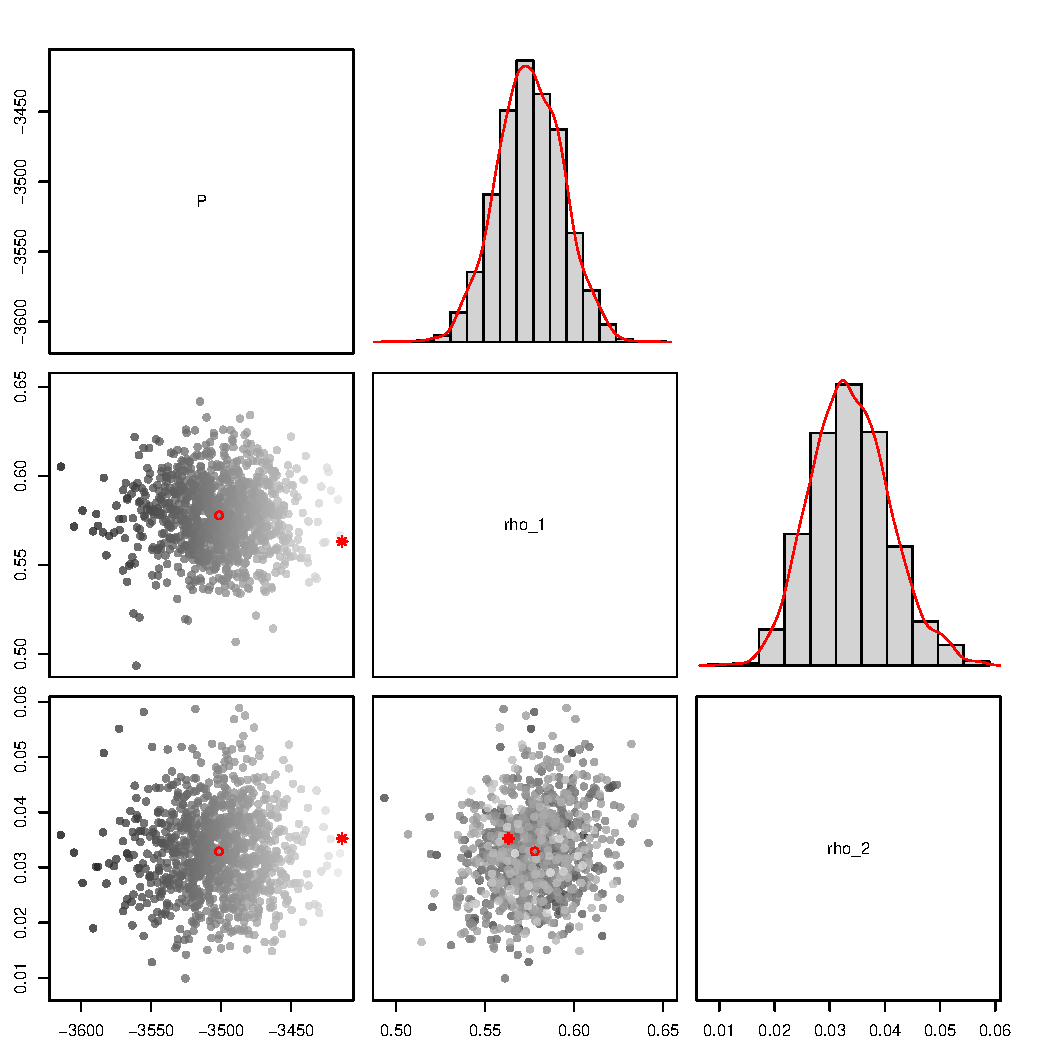
\includegraphics[page=1, width=1\linewidth]{b0_6_2/out_con/fig_postPlot_rho.pdf}
\caption{
    \textbf{Posterior distribution of the correlation parameters of the connectance model.}
    $P$ corresponds to the log posterior density of the parameters, $rho_1$ corresponds to the maximum correlation parameter (i.e. $\alpha$ in the main text), and $rho_2$ is the rate of decrease (of the correlation) with distance (i.e. $\beta$ in the main text). 
    These parameters model a decrease in the correlation in the connectances, $\rho_{ij}$, of two sites, $i$ and $j$ located in the same hydrographic basin with Euclidean distance, $\rho_{ij} = \alpha \exp\left( - \beta d_{ij}\right)$.
    Grey dots correspond to individual samples obtained by differential-evolution Monte-Carlo sampling of the posterior distribution (\cite{TerBraak2006}). 
} 

\end{center}
\end{figure}

%%
\begin{figure}[H]
\begin{center}
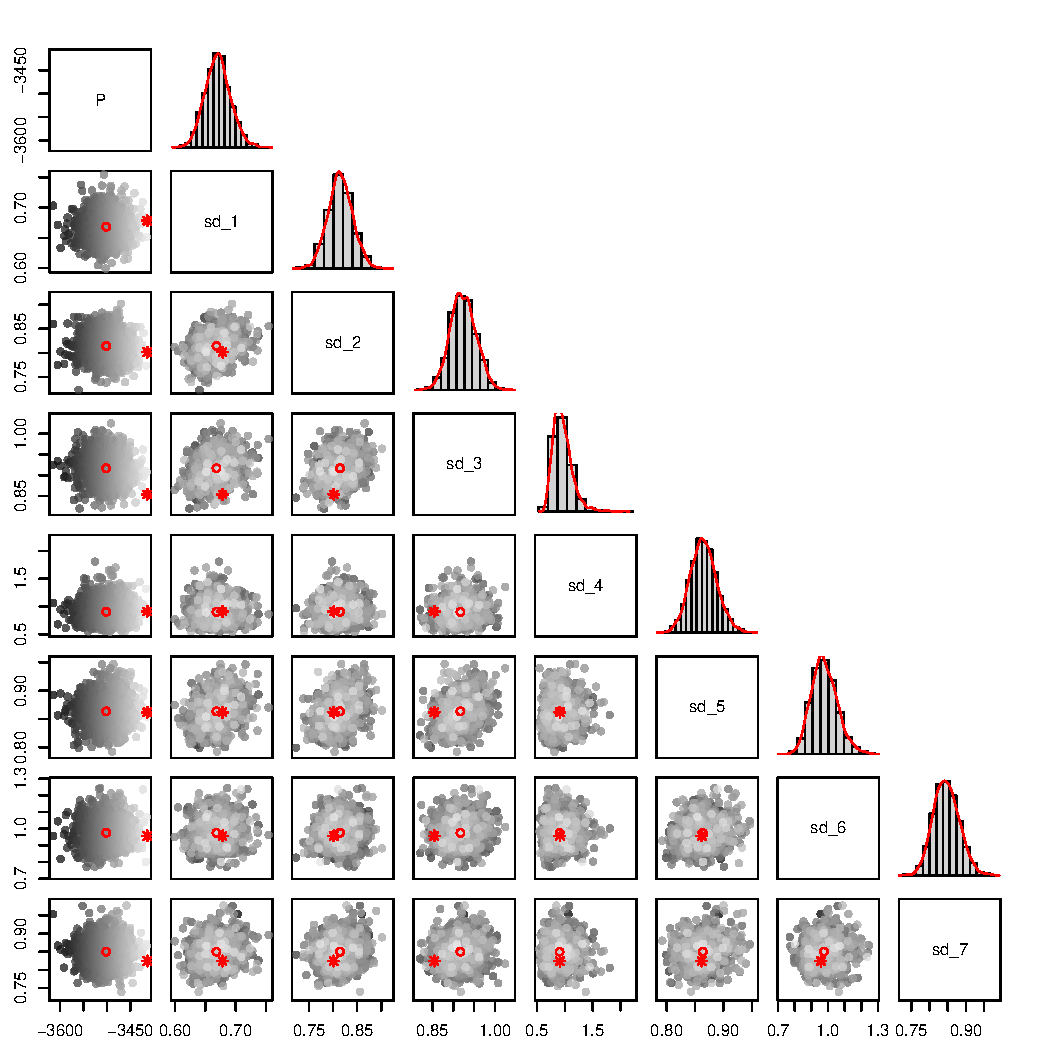
\includegraphics[page=1, width=1\linewidth]{b0_6_2/out_con/fig_postPlot_sd_lik.pdf}
\caption{
    \textbf{Posterior distribution of the standard deviations of the variance-covariance matrix of the connectance model.}
    $P$ corresponds to the log posterior density of the parameters, $sd_1$ to $sd_7$ correspond to the estimated basin-specific standard deviations of the response variable (i.e. connectance).
    Our dataset contained seven hydrographic basins, so there are seven estimated basin-specific standard deviations.
    Grey dots correspond to individual samples obtained by differential-evolution Monte-Carlo sampling of the posterior distribution (\cite{TerBraak2006}). 
    } 
\end{center}
\end{figure}

%%
\begin{figure}[H]
\begin{center}
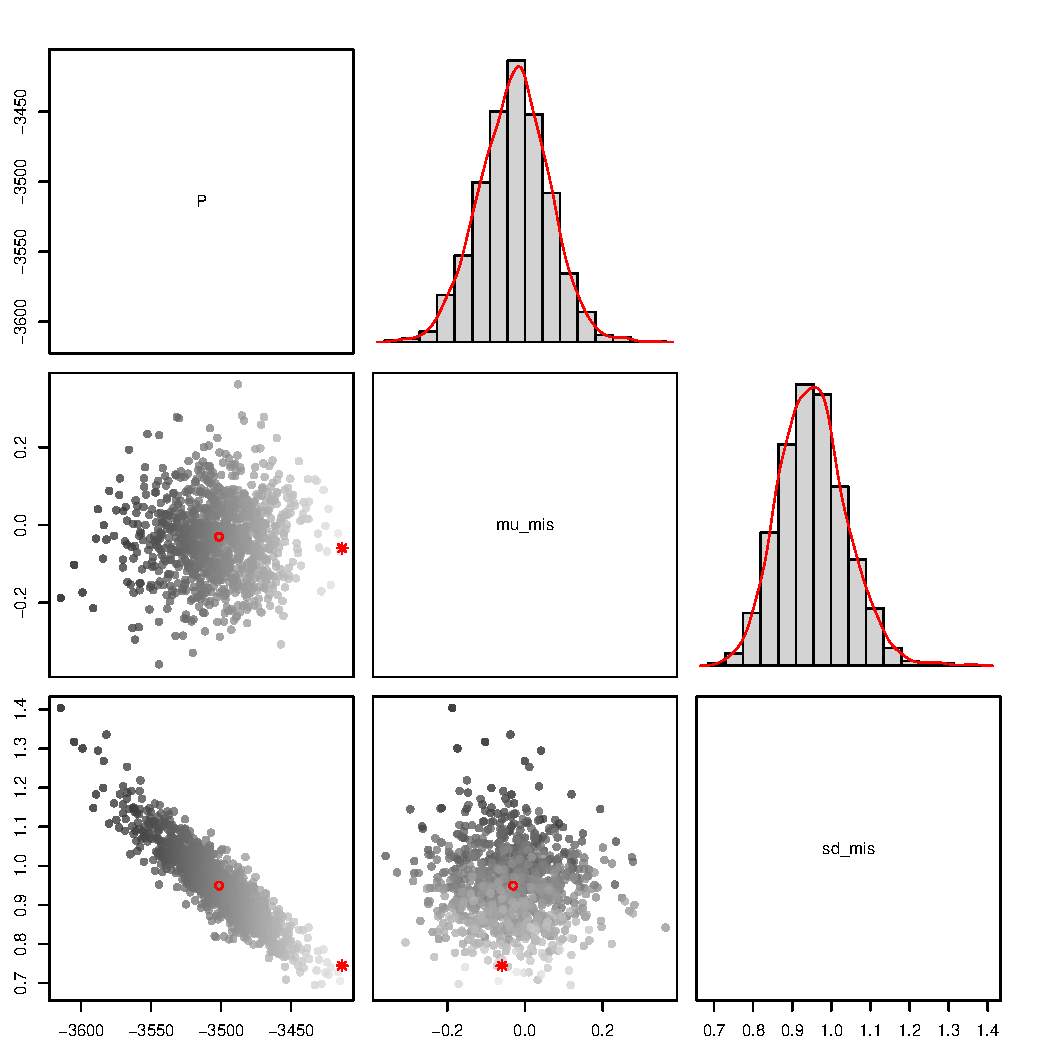
\includegraphics[page=1, width=1\linewidth]{b0_6_2/out_con/fig_postPlot_sd_mis.pdf}
\caption{
    \textbf{Posterior distribution of parameters of the distribution of missing observations of the connectance model.}
    $P$ corresponds to the log posterior density of the parameters.
    $mu_{mis}$ and $sd_{mis}$ correspond to the mean and standard deviation of the distribution of the missing BOD observations.
    The distribution of missing BOD measurements is assumed to be a normal distribution.
    Grey dots correspond to individual samples obtained by differential-evolution Monte-Carlo sampling of the posterior distribution (\cite{TerBraak2006}). 
} 
\end{center}
\end{figure}

%%
\begin{figure}[H]
\begin{center}
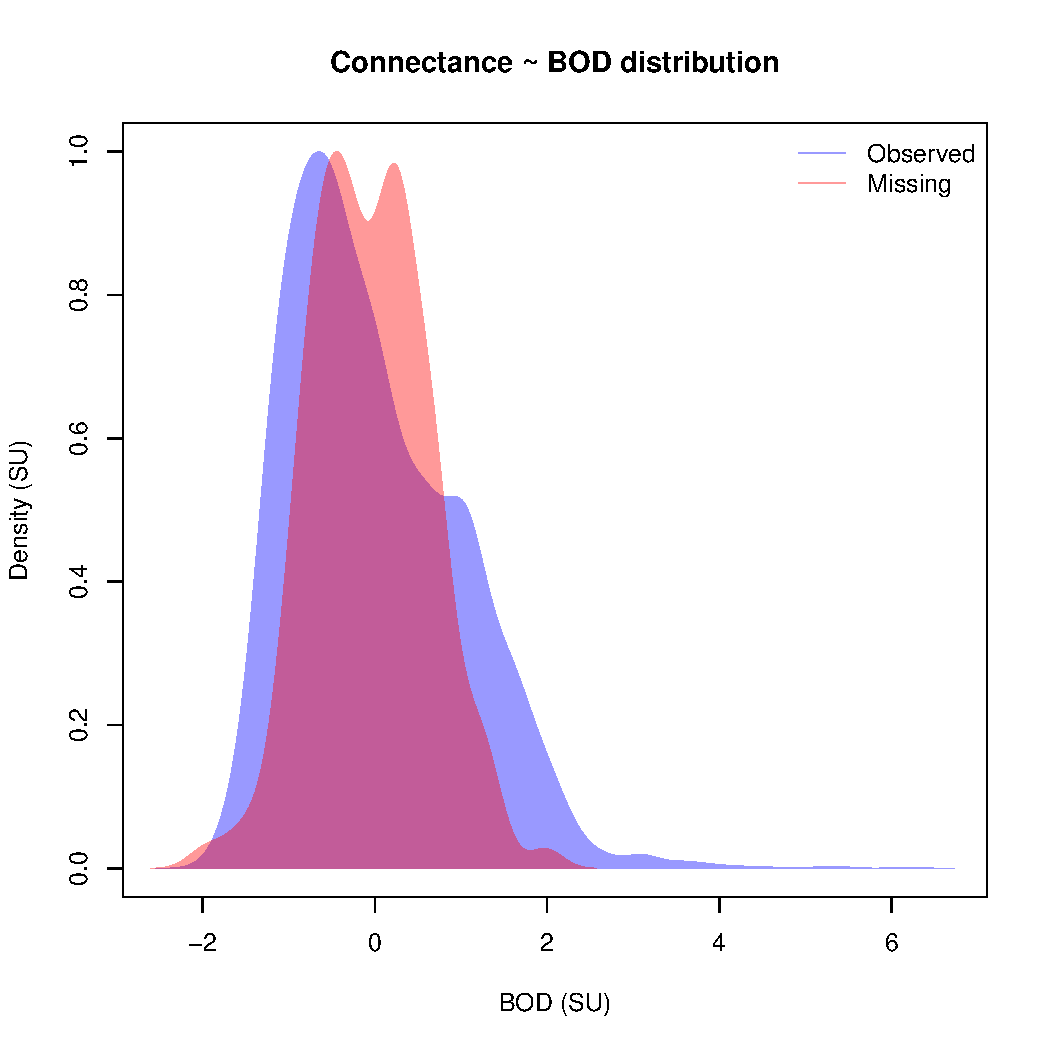
\includegraphics[page=1, width=1\linewidth]{b0_6_2/out_con/fig_hist_missing_bod.pdf}
\caption{
    \textbf{Histogram of the inferred distribution of missing BOD measurements of the connectance model.}
    The blue distribution shows the distribution of observed BOD measurements, while the red distribution shows that of missing observations, estimated by the model.
    Missing observations were estimated by differential-evolution Monte-Carlo sampling of the posterior distribution (\cite{TerBraak2006}).
    SU means standardised units, namely that the variable has been standardised by subtracting the mean and dividing by the standard deviation.
} 
\end{center}
\end{figure}

%%
\begin{figure}[H]
\begin{center}
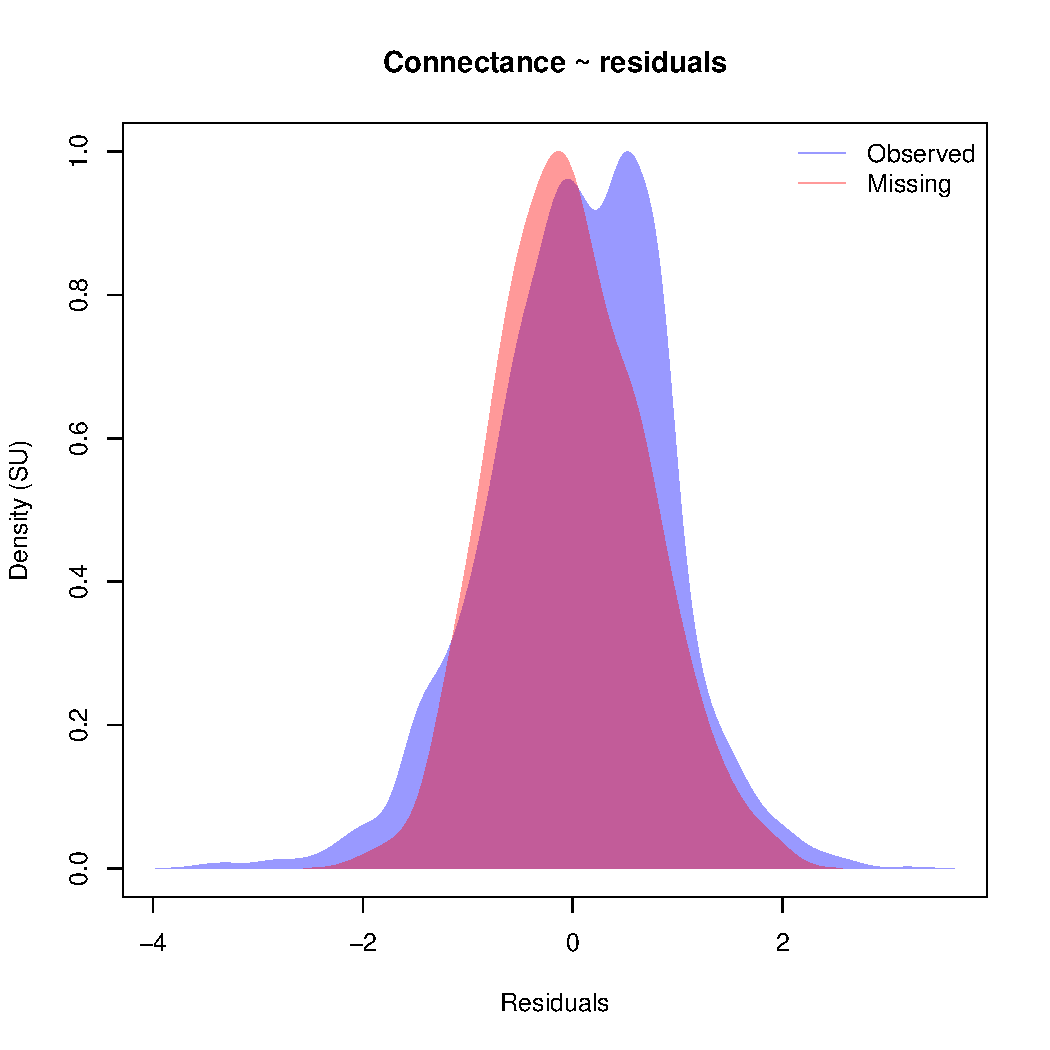
\includegraphics[page=1, width=1\linewidth]{b0_6_2/out_con/fig_hist_residuals.pdf}
\caption{
    \textbf{Histograms of the residuals of the connectance model.}
    The blue distribution corresponds to the residuals of the predictions of the model obtained where BOD observations were available, while the red distribution corresponds to residuals obtained where BOD measurements where inferred by the model.
    Missing observations were estimated by differential-evolution Monte-Carlo sampling of the posterior distribution (\cite{TerBraak2006}).
    SU means standardised units, namely that the variable has been standardised by subtracting the mean and dividing by the standard deviation.
} 
\end{center}
\end{figure}

%%
\begin{figure}[H]
\begin{center}
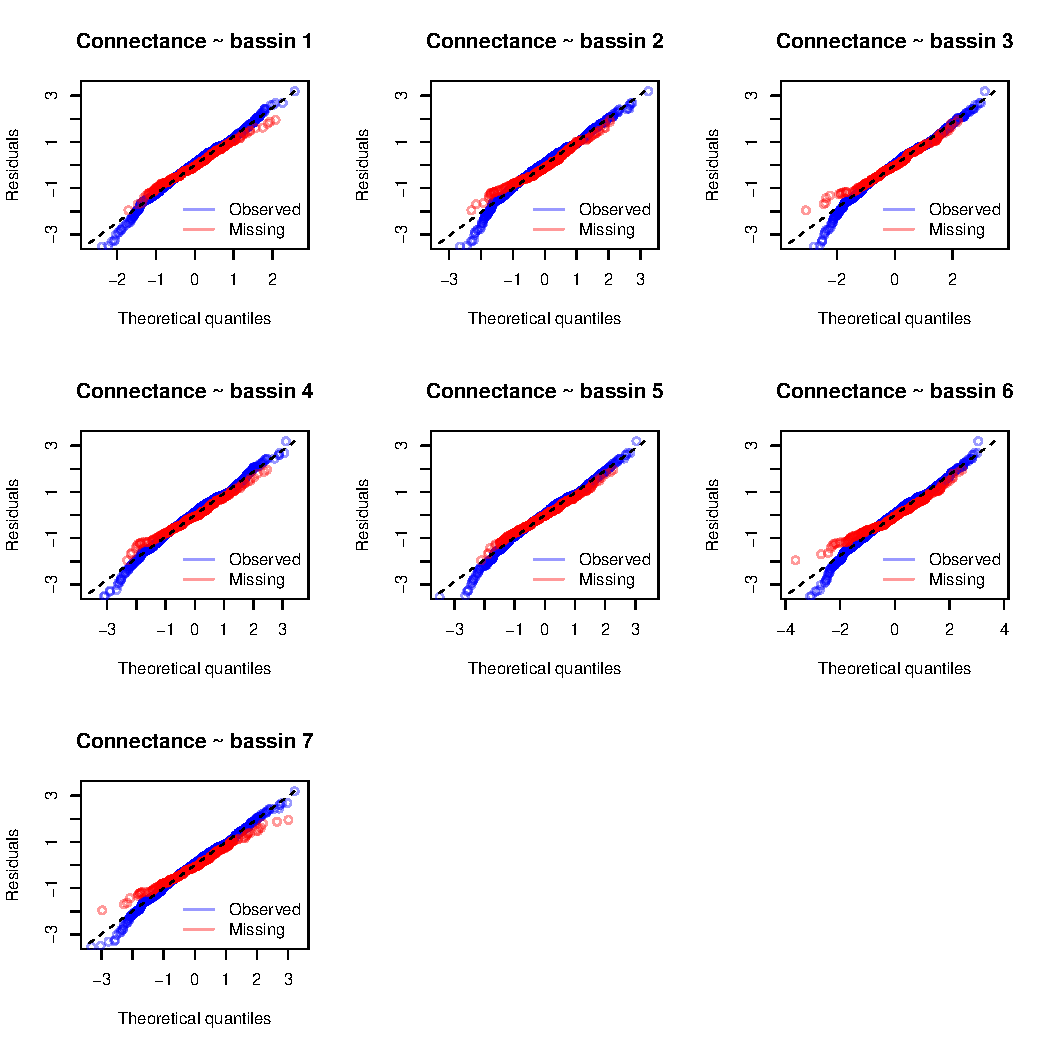
\includegraphics[page=1, width=1\linewidth]{b0_6_2/out_con/fig_qqplot_residuals.pdf}
\caption{
    \textbf{QQplots of the residuals of model predictions for each hydrographic basins.}
    The blue dots correspond to the quantiles of residuals of model predictions where BOD measurements were available, while the red dots corresponds to residuals of model predictions where BOD was estimated by the model.
    The theoretical quantiles are obtained from a normal distribution with the same mean and variance as the residuals.
} 
\end{center}
\end{figure}

%%
\begin{figure}[H]
\begin{center}
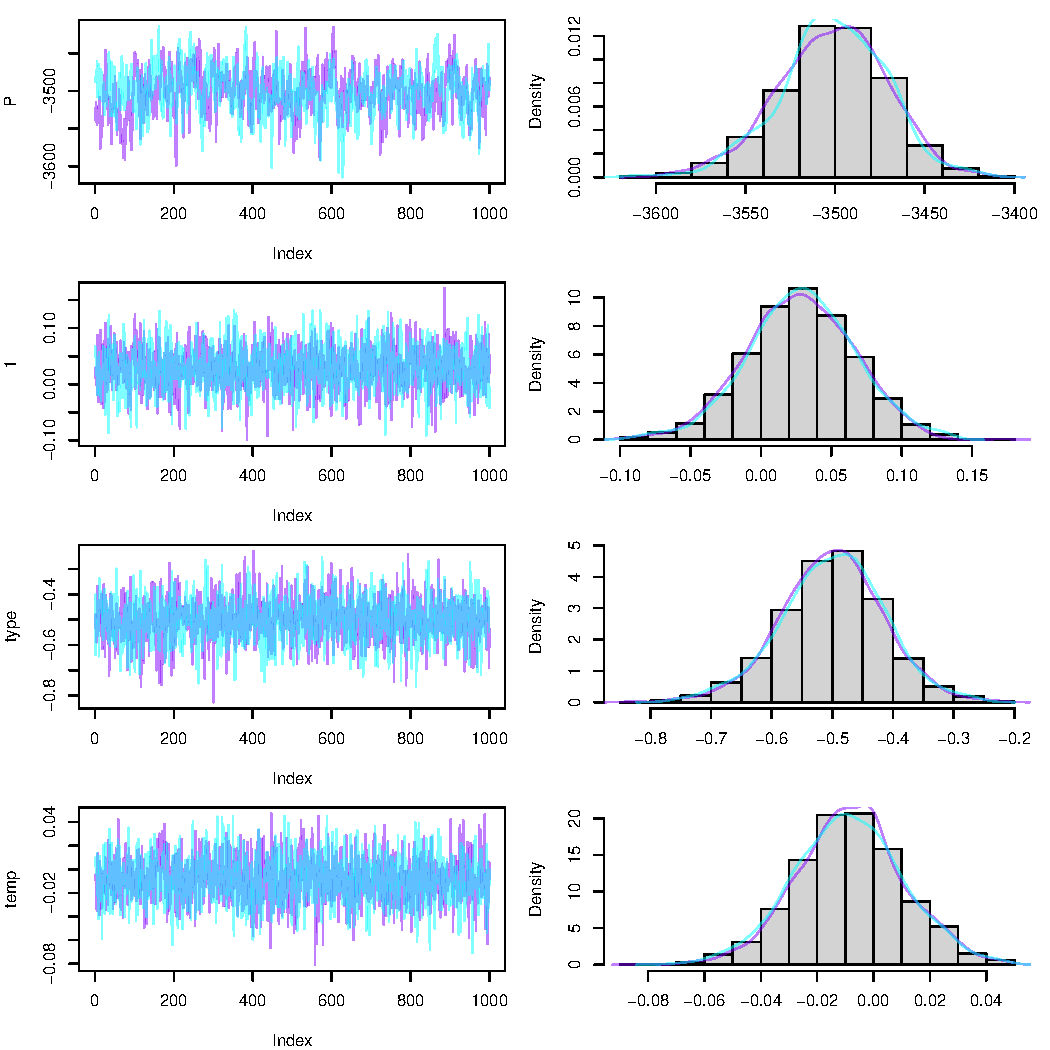
\includegraphics[page=1, width=1\linewidth]{b0_6_2/out_con/fig_tracePlot_beta.pdf}
\caption{
    \textbf{Traces of the chains of the parameters of the connectance model (1/4).}
    Each row shows samples of a given model parameter, sorted by index (left), or shown as a histogram (right).
    $P$ is the log posterior density, $1$ is the intercept, $type$ is the habitat type whether stream or lake, $temp$ is the temperature, $temp^2$ is the quadratic effect of the temperature, $temp * type$ is the interaction between temperature and habitat type, $bod$ is the biological oxygen demand, $bod^2$ is the quadratic effect of the BOD, $type * bod$ is the interaction between type and BOD, $temp * bod$ is the interaction between temperature and BOD, $temp * bod * type$ is the three-way interaction between temperature, BOD, and type, $rich$ is the trophic species richness (i.e. number of trophic species), $year$ is the year of sampling.
    Samples were obtained by differential-evolution Monte-Carlo sampling of the posterior distribution (\cite{TerBraak2006}).
    Chains were burned by removing the first half of the iterations, and then by taking a thousand evenly spaced samples of the remaining samples.
} 
\end{center}
\end{figure}

%%
\begin{figure}[H]
\begin{center}
\includegraphics[page=2, width=1\linewidth]{b0_6_2/out_con/fig_tracePlot_beta.pdf}
\caption{
    \textbf{Traces of the chains of the parameters of the connectance model (2/4).}
    Each row shows samples of a given model parameter, sorted by index (left), or shown as a histogram (right).
    $P$ is the log posterior density, $1$ is the intercept, $type$ is the habitat type whether stream or lake, $temp$ is the temperature, $temp^2$ is the quadratic effect of the temperature, $temp * type$ is the interaction between temperature and habitat type, $bod$ is the biological oxygen demand, $bod^2$ is the quadratic effect of the BOD, $type * bod$ is the interaction between type and BOD, $temp * bod$ is the interaction between temperature and BOD, $temp * bod * type$ is the three-way interaction between temperature, BOD, and type, $rich$ is the trophic species richness (i.e. number of trophic species), $year$ is the year of sampling.
    Samples were obtained by differential-evolution Monte-Carlo sampling of the posterior distribution (\cite{TerBraak2006}).
    Chains were burned by removing the first half of the iterations, and then by taking a thousand evenly spaced samples of the remaining samples.
}
\end{center}
\end{figure}

%%
\begin{figure}[H]
\begin{center}
\includegraphics[page=3, width=1\linewidth]{b0_6_2/out_con/fig_tracePlot_beta.pdf}
\caption{
    \textbf{Traces of the chains of the parameters of the connectance model (3/4).}
    Each row shows samples of a given model parameter, sorted by index (left), or shown as a histogram (right).
    $P$ is the log posterior density, $1$ is the intercept, $type$ is the habitat type whether stream or lake, $temp$ is the temperature, $temp^2$ is the quadratic effect of the temperature, $temp * type$ is the interaction between temperature and habitat type, $bod$ is the biological oxygen demand, $bod^2$ is the quadratic effect of the BOD, $type * bod$ is the interaction between type and BOD, $temp * bod$ is the interaction between temperature and BOD, $temp * bod * type$ is the three-way interaction between temperature, BOD, and type, $rich$ is the trophic species richness (i.e. number of trophic species), $year$ is the year of sampling.
    Samples were obtained by differential-evolution Monte-Carlo sampling of the posterior distribution (\cite{TerBraak2006}).
    Chains were burned by removing the first half of the iterations, and then by taking a thousand evenly spaced samples of the remaining samples.
}
\end{center}
\end{figure}

%%
\begin{figure}[H]
\begin{center}
\includegraphics[page=4, width=1\linewidth]{b0_6_2/out_con/fig_tracePlot_beta.pdf}
\caption{
    \textbf{Traces of the chains of the parameters of the connectance model (4/4).}
    Each row shows samples of a given model parameter, sorted by index (left), or shown as a histogram (right).
    $P$ is the log posterior density, $1$ is the intercept, $type$ is the habitat type whether stream or lake, $temp$ is the temperature, $temp^2$ is the quadratic effect of the temperature, $temp * type$ is the interaction between temperature and habitat type, $bod$ is the biological oxygen demand, $bod^2$ is the quadratic effect of the BOD, $type * bod$ is the interaction between type and BOD, $temp * bod$ is the interaction between temperature and BOD, $temp * bod * type$ is the three-way interaction between temperature, BOD, and type, $rich$ is the trophic species richness (i.e. number of trophic species), $year$ is the year of sampling.
    Samples were obtained by differential-evolution Monte-Carlo sampling of the posterior distribution (\cite{TerBraak2006}).
    Chains were burned by removing the first half of the iterations, and then by taking a thousand evenly spaced samples of the remaining samples.
} 
\end{center}
\end{figure}

%%
\begin{figure}[H]
\begin{center}
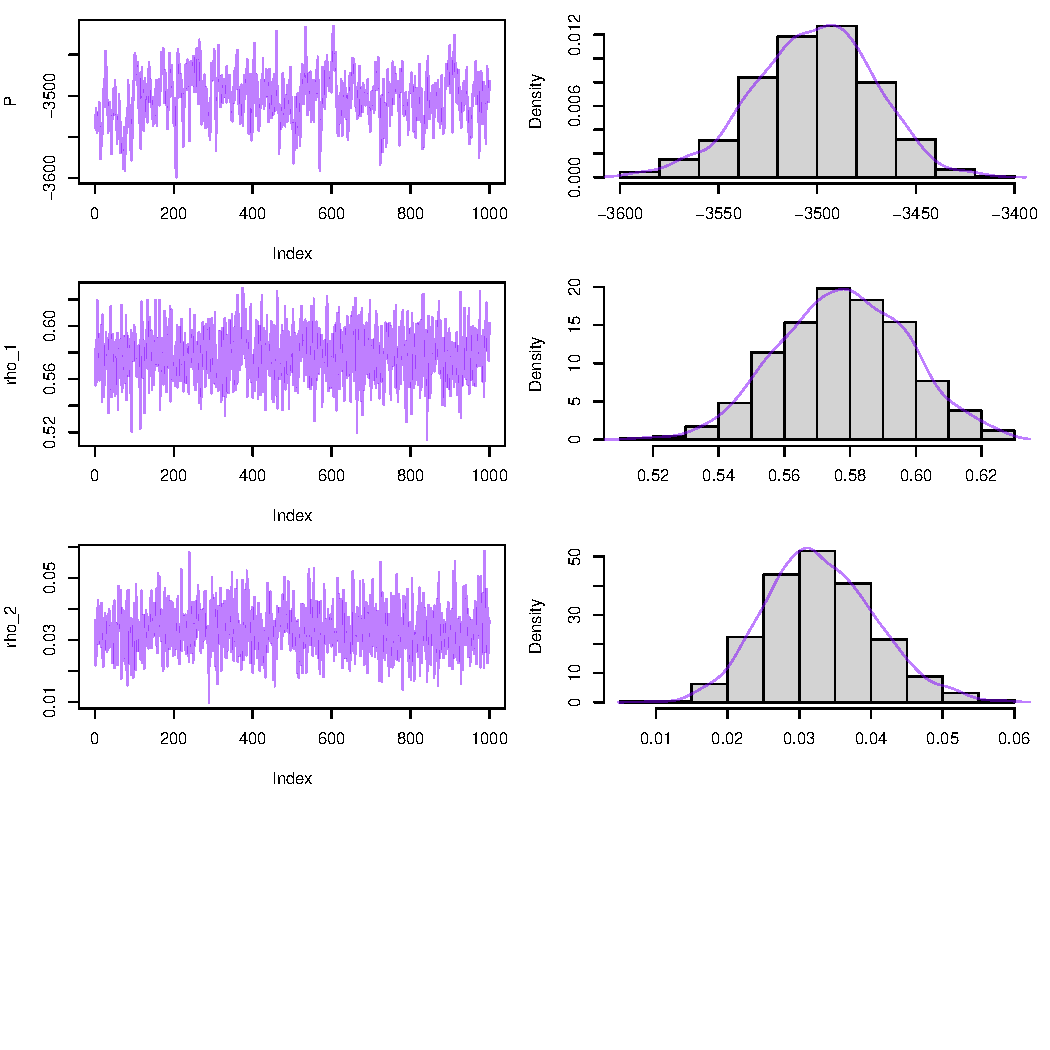
\includegraphics[page=1, width=1\linewidth]{b0_6_2/out_con/fig_tracePlot_rho.pdf}
\caption{
    \textbf{Traces of the chains of the correlation parameters of the variance-covariance matrix of the connectance model.}
    Each row shows samples of a given parameter, sorted by index (left), or shown as a histogram (right).
    $P$ corresponds to the log posterior density of the parameters, $rho_1$ corresponds to the maximum correlation parameter (i.e. $\alpha$ in the main text), and $rho_2$ is the rate of decrease (of the correlation) with distance (i.e. $\beta$ in the main text). 
    These parameters model a decrease in the correlation in the connectances, $\rho_{ij}$, of two sites, $i$ and $j$ located in the same hydrographic basin with Euclidean distance, $\rho_{ij} = \alpha \exp\left( - \beta d_{ij}\right)$.
    Samples were obtained by differential-evolution Monte-Carlo sampling of the posterior distribution (\cite{TerBraak2006}).
    Chains were burned by removing the first half of the iterations, and then by taking a thousand evenly spaced samples of the remaining samples.
} 
\end{center}
\end{figure}

%%
\begin{figure}[H]
\begin{center}
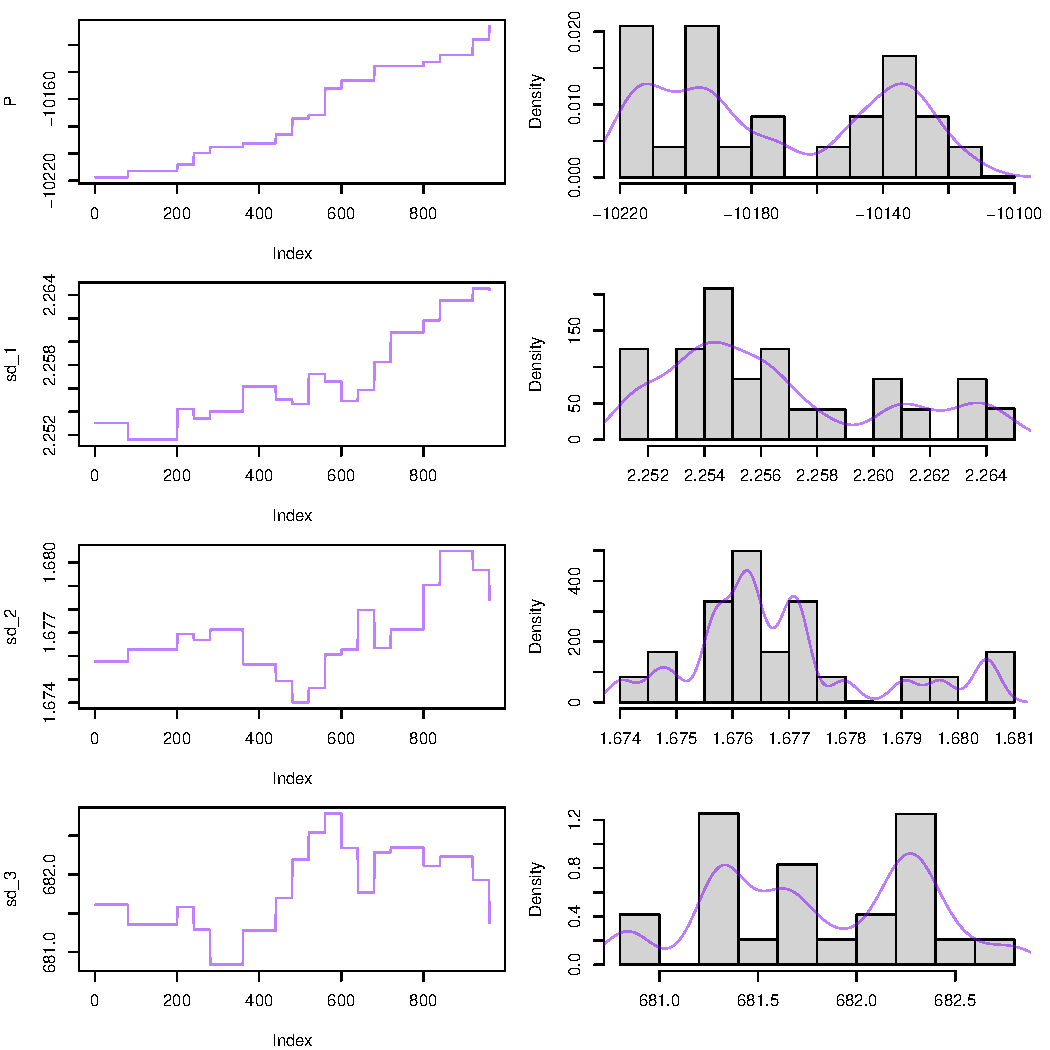
\includegraphics[page=1, width=1\linewidth]{b0_6_2/out_con/fig_tracePlot_sd_lik.pdf}
\caption{
    \textbf{Traces of the chains of the variance parameters of the variance-covariance matrix of the connectance model (1/2).}
    Each row shows samples of a given parameter, sorted by index (left), or shown as a histogram (right).
    $P$ corresponds to the log posterior density of the parameters, $sd_1$ to $sd_7$ correspond to the estimated basin-specific standard deviations of the response variable (i.e. connectance).
    Our dataset contained seven hydrographic basins, so there are seven estimated basin-specific standard deviations.
    Samples were obtained by differential-evolution Monte-Carlo sampling of the posterior distribution (\cite{TerBraak2006}).
    Chains were burned by removing the first half of the iterations, and then by taking a thousand evenly spaced samples of the remaining samples.
} 
\end{center}
\end{figure}

%%
\begin{figure}[H]
\begin{center}
\includegraphics[page=2, width=1\linewidth]{b0_6_2/out_con/fig_tracePlot_sd_lik.pdf}
\caption{
    \textbf{Traces of the chains of the variance parameters of the variance-covariance matrix of the connectance model (2/2).}
    Each row shows samples of a given parameter, sorted by index (left), or shown as a histogram (right).
    $P$ corresponds to the log posterior density of the parameters, $sd_1$ to $sd_7$ correspond to the estimated basin-specific standard deviations of the response variable (i.e. connectance).
    Our dataset contained seven hydrographic basins, so there are seven estimated basin-specific standard deviations.
    Samples were obtained by differential-evolution Monte-Carlo sampling of the posterior distribution (\cite{TerBraak2006}).
    Chains were burned by removing the first half of the iterations, and then by taking a thousand evenly spaced samples of the remaining samples.
} 
\end{center}
\end{figure}

%%
\begin{figure}[H]
\begin{center}
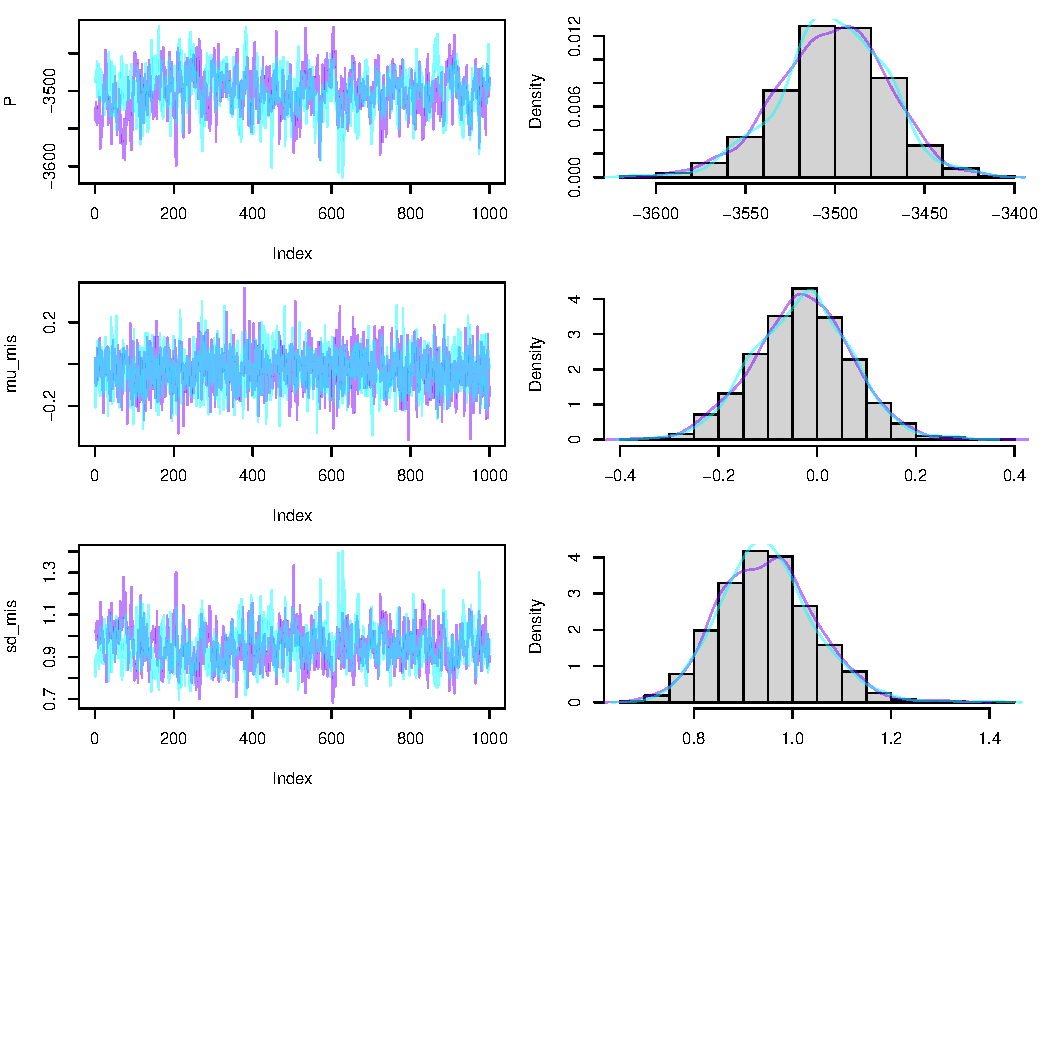
\includegraphics[page=1, width=1\linewidth]{b0_6_2/out_con/fig_tracePlot_sd_mis.pdf}
\caption{
    \textbf{Traces of the chains of the parameters of the distribution of missing BOD measurements of the connectance model.}
    Each row shows samples of a given parameter, sorted by index (left), or shown as a histogram (right).
    $P$ corresponds to the log posterior density of the parameters.
    $mu_{mis}$ and $sd_{mis}$ correspond to the mean and standard deviation of the distribution of the missing BOD observations.
    The distribution of missing BOD measurements is assumed to be a normal distribution.
    Samples were obtained by differential-evolution Monte-Carlo sampling of the posterior distribution (\cite{TerBraak2006}).
    Chains were burned by removing the first half of the iterations, and then by taking a thousand evenly spaced samples of the remaining samples.
} 
\end{center}
\end{figure}

%%
\newpage
\section{Maximum trophic level model}

%%
\begin{table}[H]
    \caption{
        \textbf{Summary table of estimated parameters for the maximum trophic level model.}
        The column name shows the terms included in the linear predictive function $\hat{Y}$ of the model and the log posterior density, denoted $\log P$.
        The MaP, mean, and sd, column correspond to the maximum \textit{a posteriori} (i.e. the value that maximises the log-posterior density), mean, and standard deviation of each term, estimated from the chains.
        The quantities $q_{05}, q_{50}, q_{95}$ correspond to the $5\%$, $50\%$, and $95\%$ quantiles of the estimated distribution of each term.
        The quantity $\hat{r}$ refers to the convergence index (\cite{Gelman1995}), which indicates whether the chains have converged or not.
        The significativity column shows whether the $90\%$ confidence interval of a given term excludes 0 or not.
    }
    \begin{center}
    \begin{tabular}{lcccccccc}
        \hline
        \\
        name & max & mean & sd & $q_{05}$ & $q_{50}$ & $q_{95}$ & $\hat{r}$ & signif. \\
        \\
        \hline
        \\
        $P$ & -3314.9016 & -3408.5997 & 31.7737 & -3461.2203 & -3408.3663 & -3354.8131 & 1.006 & * \\
        $1$ & -0.005 & -0.0144 & 0.0422 & -0.0816 & -0.0156 & 0.0547 & 0.999 & ns \\
        $type$ & 0.7109 & 0.8017 & 0.0848 & 0.6619 & 0.803 & 0.9411 & 0.9998 & * \\
        $temp$ & -0.0199 & -0.0145 & 0.0196 & -0.047 & -0.0149 & 0.0176 & 0.9999 & ns \\
        $temp^2$ & -0.0211 & -0.018 & 0.0075 & -0.0306 & -0.0177 & -0.0061 & 1.0001 & * \\
        $temp*type$ & 0.0361 & 0.007 & 0.0627 & -0.0936 & 0.006 & 0.1109 & 0.9995 & ns \\
        $bod$ & 1e-04 & -0.0103 & 0.0203 & -0.0438 & -0.0102 & 0.0234 & 0.9999 & ns \\
        $bod^2$ & -0.0172 & -0.0055 & 0.0086 & -0.0195 & -0.0055 & 0.0084 & 1.0008 & ns \\
        $type*bod$ & 0.0972 & 0.0045 & 0.1087 & -0.1761 & 0.0114 & 0.1783 & 0.9999 & ns \\
        $temp*bod$ & -0.0547 & -0.0431 & 0.0149 & -0.0678 & -0.043 & -0.0186 & 1.0019 & * \\
        $temp*bod*type$ & -0.0688 & -0.0544 & 0.0858 & -0.1874 & -0.0561 & 0.0886 & 0.999 & ns \\
        $rich$ & 0.1854 & 0.2125 & 0.0239 & 0.1732 & 0.2124 & 0.2513 & 1.0004 & * \\
        $year$ & -0.0186 & -0.0145 & 0.0126 & -0.0355 & -0.0144 & 0.006 & 0.9994 & ns \\
    \end{tabular}
    \end{center}
\end{table}

%%
\begin{figure}[H]
\begin{center}
\includegraphics[page=1, width=1\linewidth]{b0_6_2/out_mTL/fig_postPlot_beta.pdf}
\caption{
    \textbf{Posterior distribution of model parameters of the maximum trophic level model.}
    In order: $P$ is the log posterior density, $1$ is the intercept, $type$ is the habitat type whether stream or lake, $temp$ is the temperature, $temp^2$ is the quadratic effect of the temperature, $temp * type$ is the interaction between temperature and habitat type, $bod$ is the biological oxygen demand, $bod^2$ is the quadratic effect of the BOD, $type * bod$ is the interaction between type and BOD, $temp * bod$ is the interaction between temperature and BOD, $temp * bod * type$ is the three-way interaction between temperature, BOD, and type, $rich$ is the trophic species richness (i.e. number of trophic species), $year$ is the year of sampling.
    Grey dots correspond to individual samples obtained by differential-evolution Monte-Carlo sampling of the posterior distribution (\cite{TerBraak2006}). 
} 
\end{center}
\end{figure}

%%
\begin{figure}[H]
\begin{center}
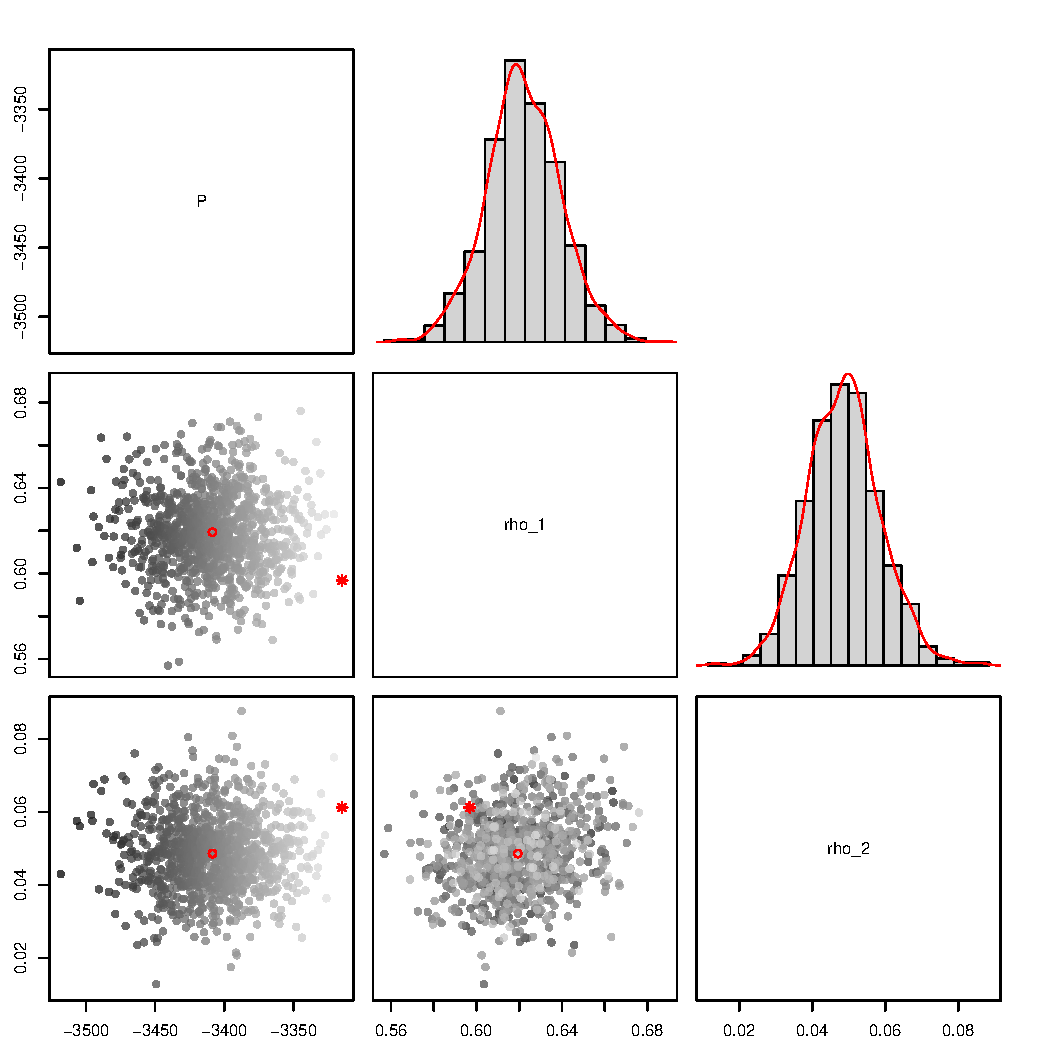
\includegraphics[page=1, width=1\linewidth]{b0_6_2/out_mTL/fig_postPlot_rho.pdf}
\caption{
    \textbf{Posterior distribution of the correlation parameters of the maximum trophic level model.}
    $P$ corresponds to the log posterior density of the parameters, $rho_1$ corresponds to the maximum correlation parameter (i.e. $\alpha$ in the main text), and $rho_2$ is the rate of decrease (of the correlation) with distance (i.e. $\beta$ in the main text). 
    These parameters model a decrease in the correlation in the maximum trophic levels, $\rho_{ij}$, of two sites, $i$ and $j$ located in the same hydrographic basin with Euclidean distance, $\rho_{ij} = \alpha \exp\left( - \beta d_{ij}\right)$.
    Grey dots correspond to individual samples obtained by differential-evolution Monte-Carlo sampling of the posterior distribution (\cite{TerBraak2006}). 
} 

\end{center}
\end{figure}

%%
\begin{figure}[H]
\begin{center}
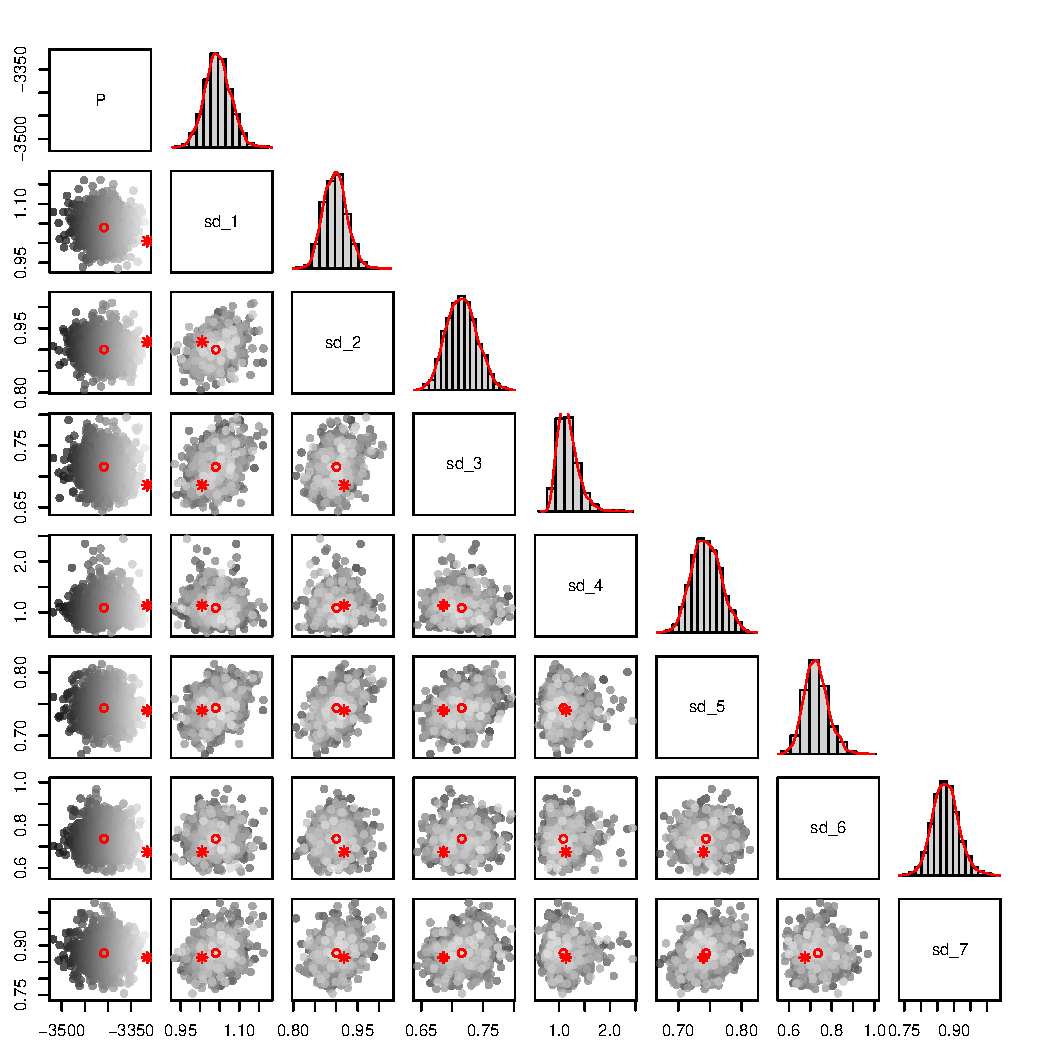
\includegraphics[page=1, width=1\linewidth]{b0_6_2/out_mTL/fig_postPlot_sd_lik.pdf}
\caption{
    \textbf{Posterior distribution of the standard deviations of the variance-covariance matrix of the maximum trophic level model.}
    $P$ corresponds to the log posterior density of the parameters, $sd_1$ to $sd_7$ correspond to the estimated basin-specific standard deviations of the response variable (i.e. maximum trophic level).
    Our dataset contained seven hydrographic basins, so there are seven estimated basin-specific standard deviations.
    Grey dots correspond to individual samples obtained by differential-evolution Monte-Carlo sampling of the posterior distribution (\cite{TerBraak2006}). 
    } 
\end{center}
\end{figure}

%%
\begin{figure}[H]
\begin{center}
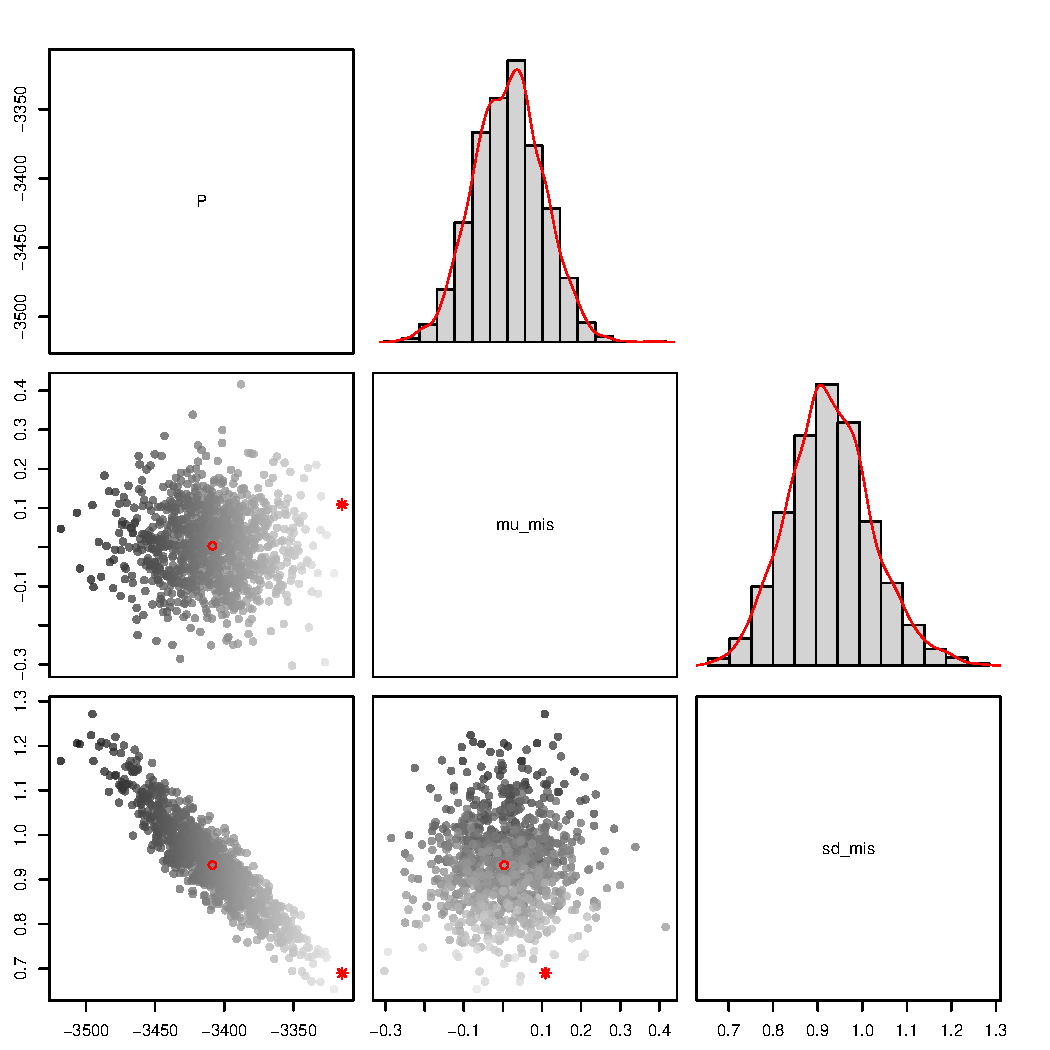
\includegraphics[page=1, width=1\linewidth]{b0_6_2/out_mTL/fig_postPlot_sd_mis.pdf}
\caption{
    \textbf{Posterior distribution of parameters of the distribution of missing observations of the maximum trophic level model.}
    $P$ corresponds to the log posterior density of the parameters.
    $mu_{mis}$ and $sd_{mis}$ correspond to the mean and standard deviation of the distribution of the missing BOD observations.
    The distribution of missing BOD measurements is assumed to be a normal distribution.
    Grey dots correspond to individual samples obtained by differential-evolution Monte-Carlo sampling of the posterior distribution (\cite{TerBraak2006}). 
} 
\end{center}
\end{figure}

%%
\begin{figure}[H]
\begin{center}
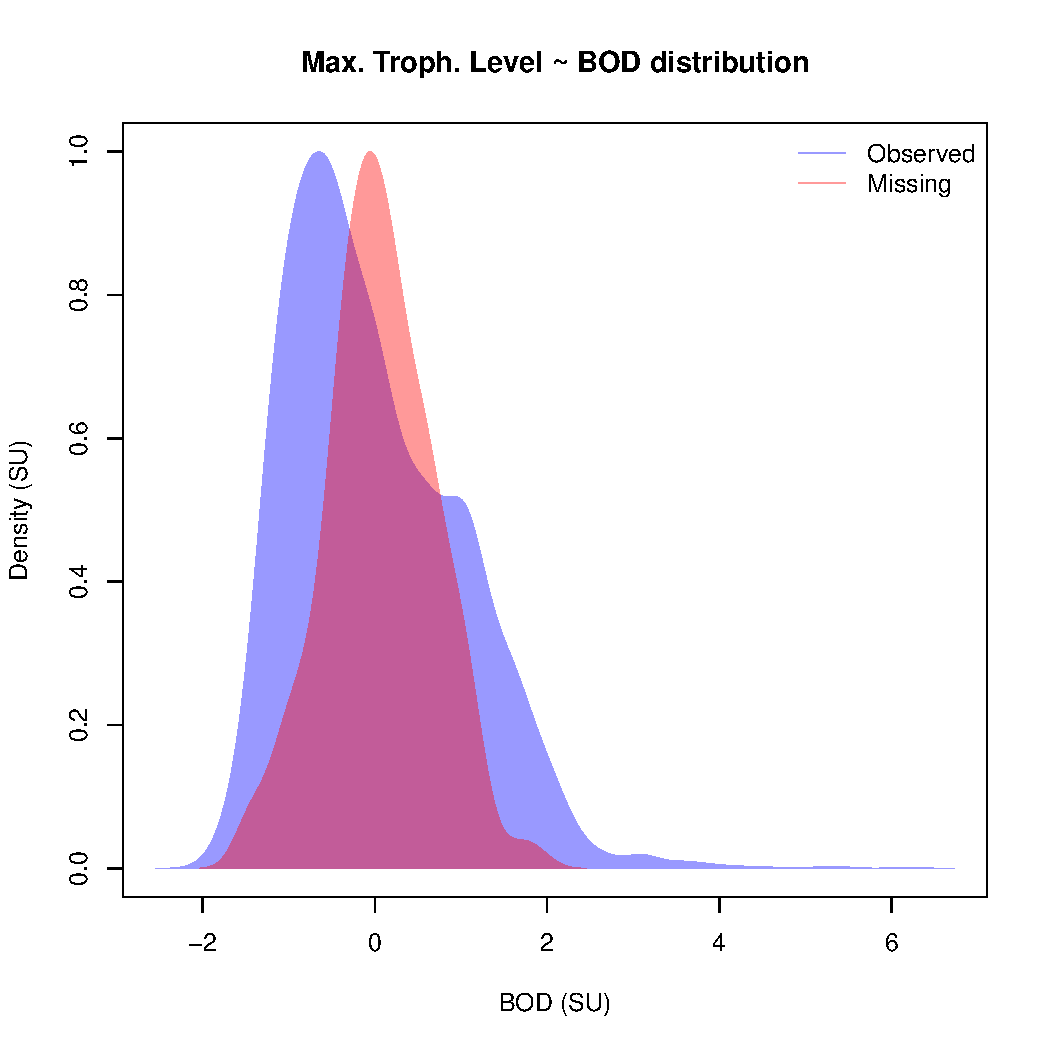
\includegraphics[page=1, width=1\linewidth]{b0_6_2/out_mTL/fig_hist_missing_bod.pdf}
\caption{
    \textbf{Histogram of the inferred distribution of missing BOD measurements of the maximum trophic level model.}
    The blue distribution shows the distribution of observed BOD measurements, while the red distribution shows that of missing observations, estimated by the model.
    Missing observations were estimated by differential-evolution Monte-Carlo sampling of the posterior distribution (\cite{TerBraak2006}).
    SU means standardised units, namely that the variable has been standardised by subtracting the mean and dividing by the standard deviation.
} 
\end{center}
\end{figure}

%%
\begin{figure}[H]
\begin{center}
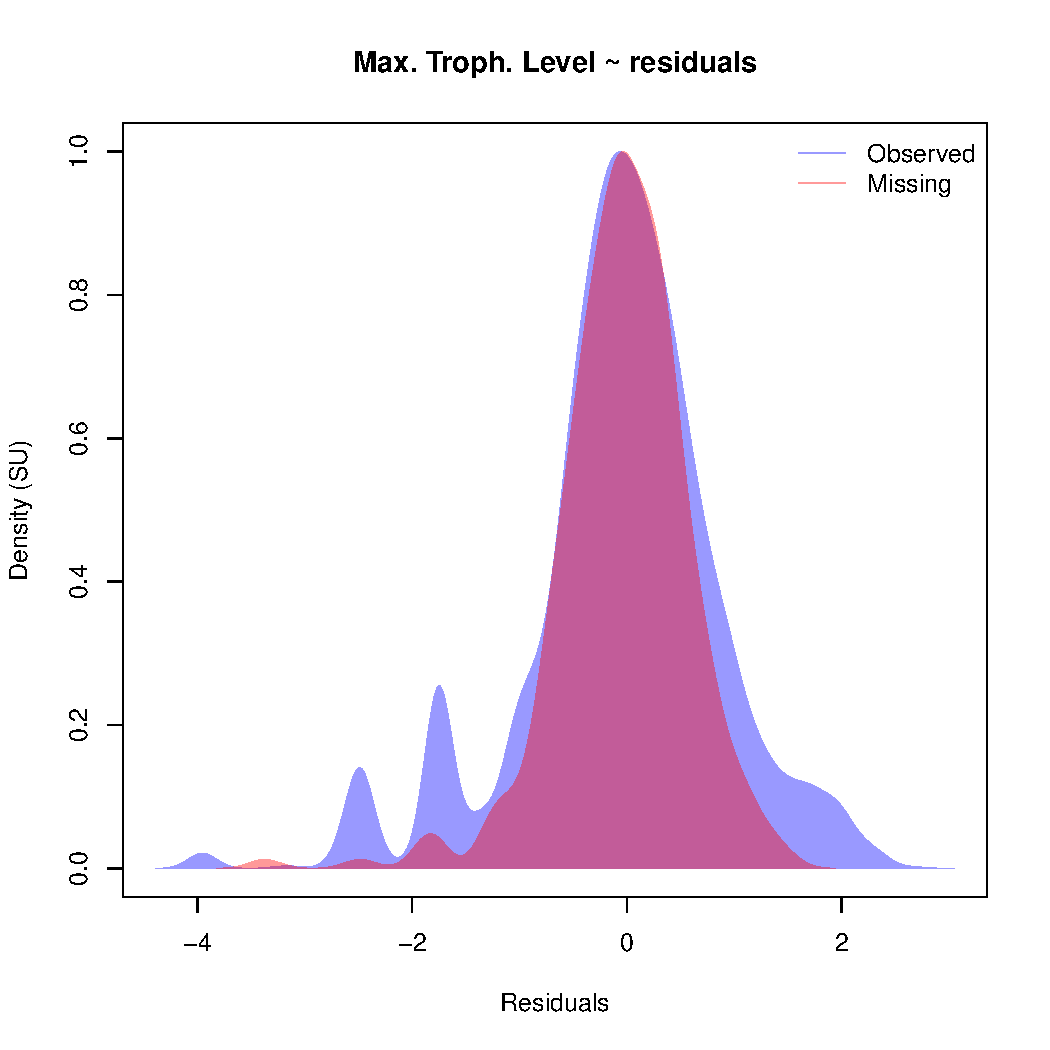
\includegraphics[page=1, width=1\linewidth]{b0_6_2/out_mTL/fig_hist_residuals.pdf}
\caption{
    \textbf{Histograms of the residuals of the maximum trophic level model.}
    The blue distribution corresponds to the residuals of the predictions of the model obtained where BOD observations were available, while the red distribution corresponds to residuals obtained where BOD measurements where inferred by the model.
    Missing observations were estimated by differential-evolution Monte-Carlo sampling of the posterior distribution (\cite{TerBraak2006}).
    SU means standardised units, namely that the variable has been standardised by subtracting the mean and dividing by the standard deviation.
} 
\end{center}
\end{figure}

%%
\begin{figure}[H]
\begin{center}
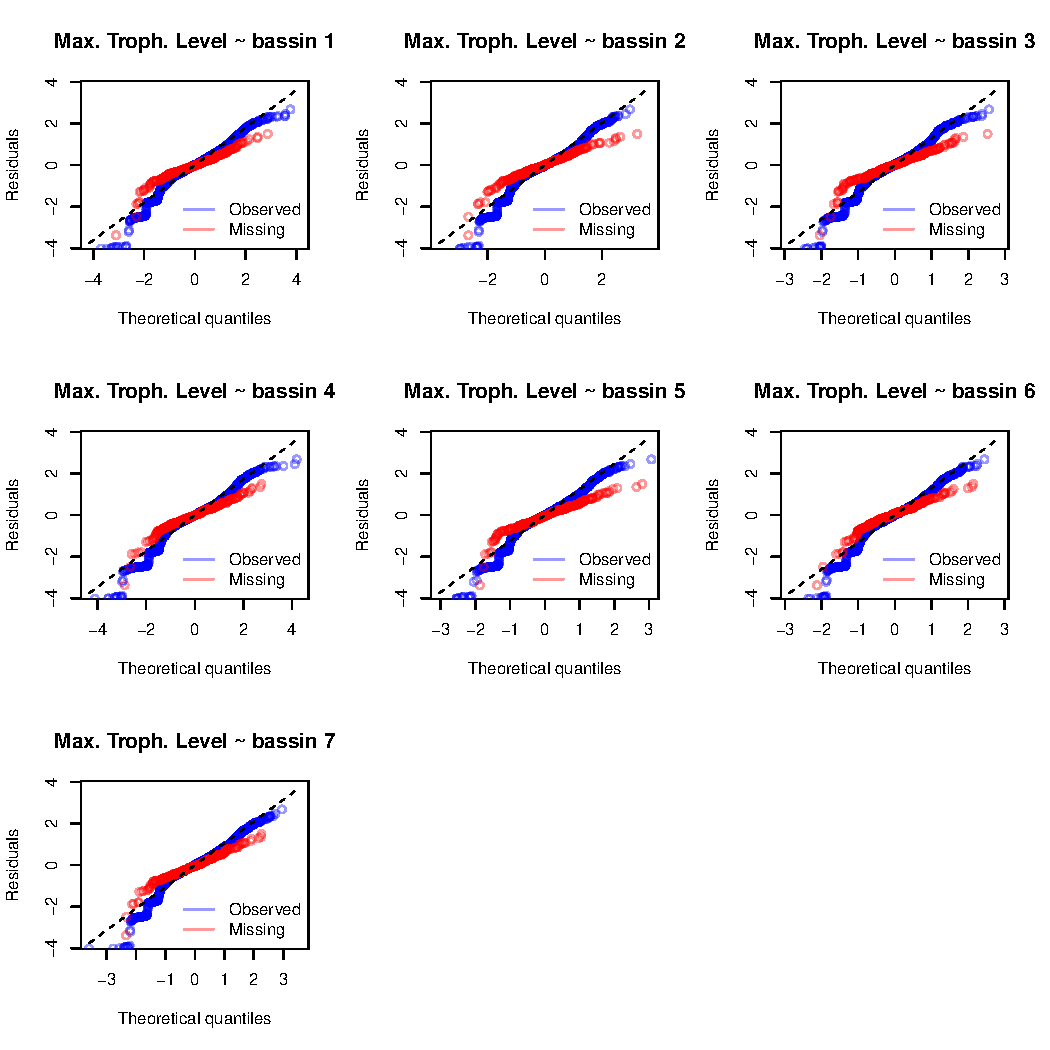
\includegraphics[page=1, width=1\linewidth]{b0_6_2/out_mTL/fig_qqplot_residuals.pdf}
\caption{
    \textbf{QQplots of the residuals of model predictions for each hydrographic basins.}
    The blue dots correspond to the quantiles of residuals of model predictions where BOD measurements were available, while the red dots corresponds to residuals of model predictions where BOD was estimated by the model.
    The theoretical quantiles are obtained from a normal distribution with the same mean and variance as the residuals.
} 
\end{center}
\end{figure}

%%
\begin{figure}[H]
\begin{center}
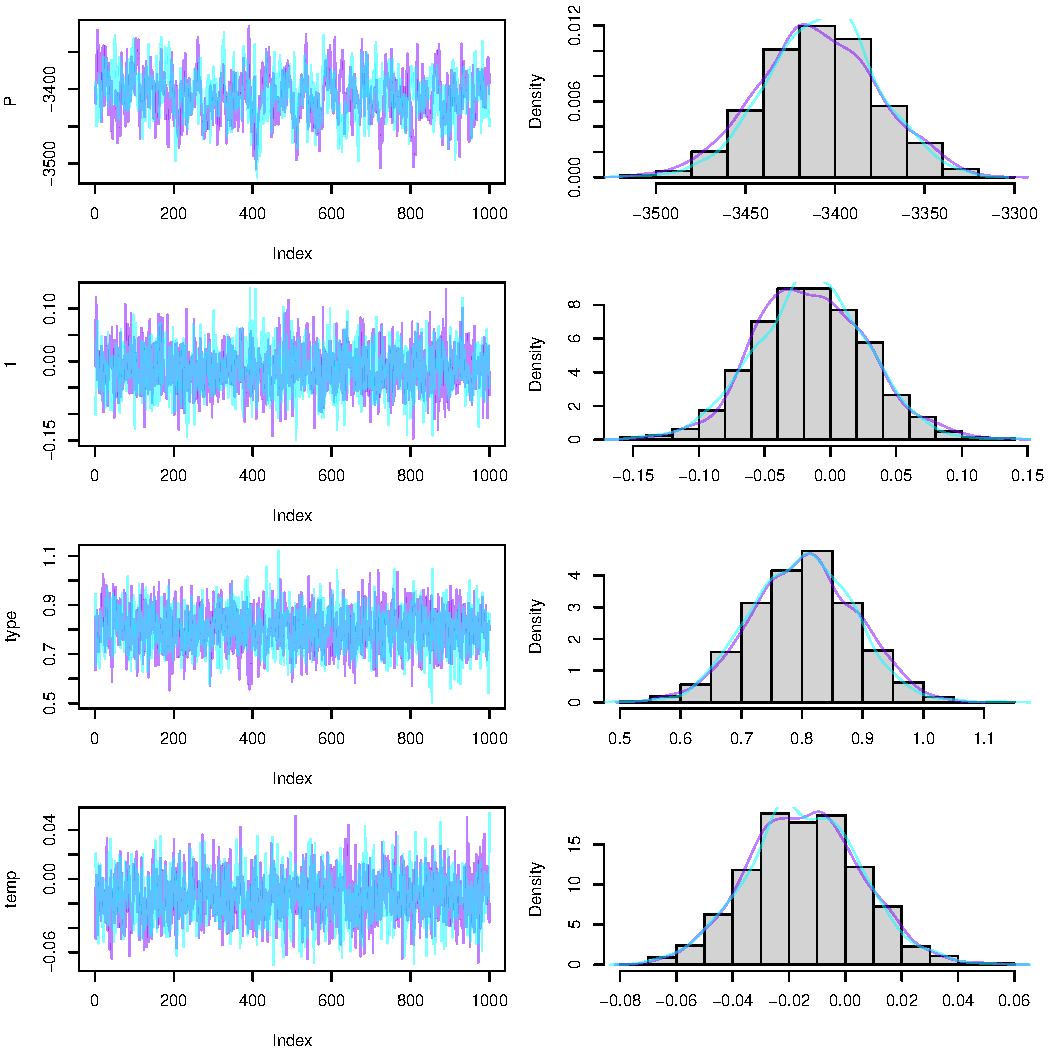
\includegraphics[page=1, width=1\linewidth]{b0_6_2/out_mTL/fig_tracePlot_beta.pdf}
\caption{
    \textbf{Traces of the chains of the parameters of the maximum trophic level model (1/4).}
    Each row shows samples of a given model parameter, sorted by index (left), or shown as a histogram (right).
    $P$ is the log posterior density, $1$ is the intercept, $type$ is the habitat type whether stream or lake, $temp$ is the temperature, $temp^2$ is the quadratic effect of the temperature, $temp * type$ is the interaction between temperature and habitat type, $bod$ is the biological oxygen demand, $bod^2$ is the quadratic effect of the BOD, $type * bod$ is the interaction between type and BOD, $temp * bod$ is the interaction between temperature and BOD, $temp * bod * type$ is the three-way interaction between temperature, BOD, and type, $rich$ is the trophic species richness (i.e. number of trophic species), $year$ is the year of sampling.
    Samples were obtained by differential-evolution Monte-Carlo sampling of the posterior distribution (\cite{TerBraak2006}).
    Chains were burned by removing the first half of the iterations, and then by taking a thousand evenly spaced samples of the remaining samples.
} 
\end{center}
\end{figure}

%%
\begin{figure}[H]
\begin{center}
\includegraphics[page=2, width=1\linewidth]{b0_6_2/out_mTL/fig_tracePlot_beta.pdf}
\caption{
    \textbf{Traces of the chains of the parameters of the maximum trophic level model (2/4).}
    Each row shows samples of a given model parameter, sorted by index (left), or shown as a histogram (right).
    $P$ is the log posterior density, $1$ is the intercept, $type$ is the habitat type whether stream or lake, $temp$ is the temperature, $temp^2$ is the quadratic effect of the temperature, $temp * type$ is the interaction between temperature and habitat type, $bod$ is the biological oxygen demand, $bod^2$ is the quadratic effect of the BOD, $type * bod$ is the interaction between type and BOD, $temp * bod$ is the interaction between temperature and BOD, $temp * bod * type$ is the three-way interaction between temperature, BOD, and type, $rich$ is the trophic species richness (i.e. number of trophic species), $year$ is the year of sampling.
    Samples were obtained by differential-evolution Monte-Carlo sampling of the posterior distribution (\cite{TerBraak2006}).
    Chains were burned by removing the first half of the iterations, and then by taking a thousand evenly spaced samples of the remaining samples.
}
\end{center}
\end{figure}

%%
\begin{figure}[H]
\begin{center}
\includegraphics[page=3, width=1\linewidth]{b0_6_2/out_mTL/fig_tracePlot_beta.pdf}
\caption{
    \textbf{Traces of the chains of the parameters of the maximum trophic level model (3/4).}
    Each row shows samples of a given model parameter, sorted by index (left), or shown as a histogram (right).
    $P$ is the log posterior density, $1$ is the intercept, $type$ is the habitat type whether stream or lake, $temp$ is the temperature, $temp^2$ is the quadratic effect of the temperature, $temp * type$ is the interaction between temperature and habitat type, $bod$ is the biological oxygen demand, $bod^2$ is the quadratic effect of the BOD, $type * bod$ is the interaction between type and BOD, $temp * bod$ is the interaction between temperature and BOD, $temp * bod * type$ is the three-way interaction between temperature, BOD, and type, $rich$ is the trophic species richness (i.e. number of trophic species), $year$ is the year of sampling.
    Samples were obtained by differential-evolution Monte-Carlo sampling of the posterior distribution (\cite{TerBraak2006}).
    Chains were burned by removing the first half of the iterations, and then by taking a thousand evenly spaced samples of the remaining samples.
}
\end{center}
\end{figure}

%%
\begin{figure}[H]
\begin{center}
\includegraphics[page=4, width=1\linewidth]{b0_6_2/out_mTL/fig_tracePlot_beta.pdf}
\caption{
    \textbf{Traces of the chains of the parameters of the maximum trophic level model (4/4).}
    Each row shows samples of a given model parameter, sorted by index (left), or shown as a histogram (right).
    $P$ is the log posterior density, $1$ is the intercept, $type$ is the habitat type whether stream or lake, $temp$ is the temperature, $temp^2$ is the quadratic effect of the temperature, $temp * type$ is the interaction between temperature and habitat type, $bod$ is the biological oxygen demand, $bod^2$ is the quadratic effect of the BOD, $type * bod$ is the interaction between type and BOD, $temp * bod$ is the interaction between temperature and BOD, $temp * bod * type$ is the three-way interaction between temperature, BOD, and type, $rich$ is the trophic species richness (i.e. number of trophic species), $year$ is the year of sampling.
    Samples were obtained by differential-evolution Monte-Carlo sampling of the posterior distribution (\cite{TerBraak2006}).
    Chains were burned by removing the first half of the iterations, and then by taking a thousand evenly spaced samples of the remaining samples.
} 
\end{center}
\end{figure}

%%
\begin{figure}[H]
\begin{center}
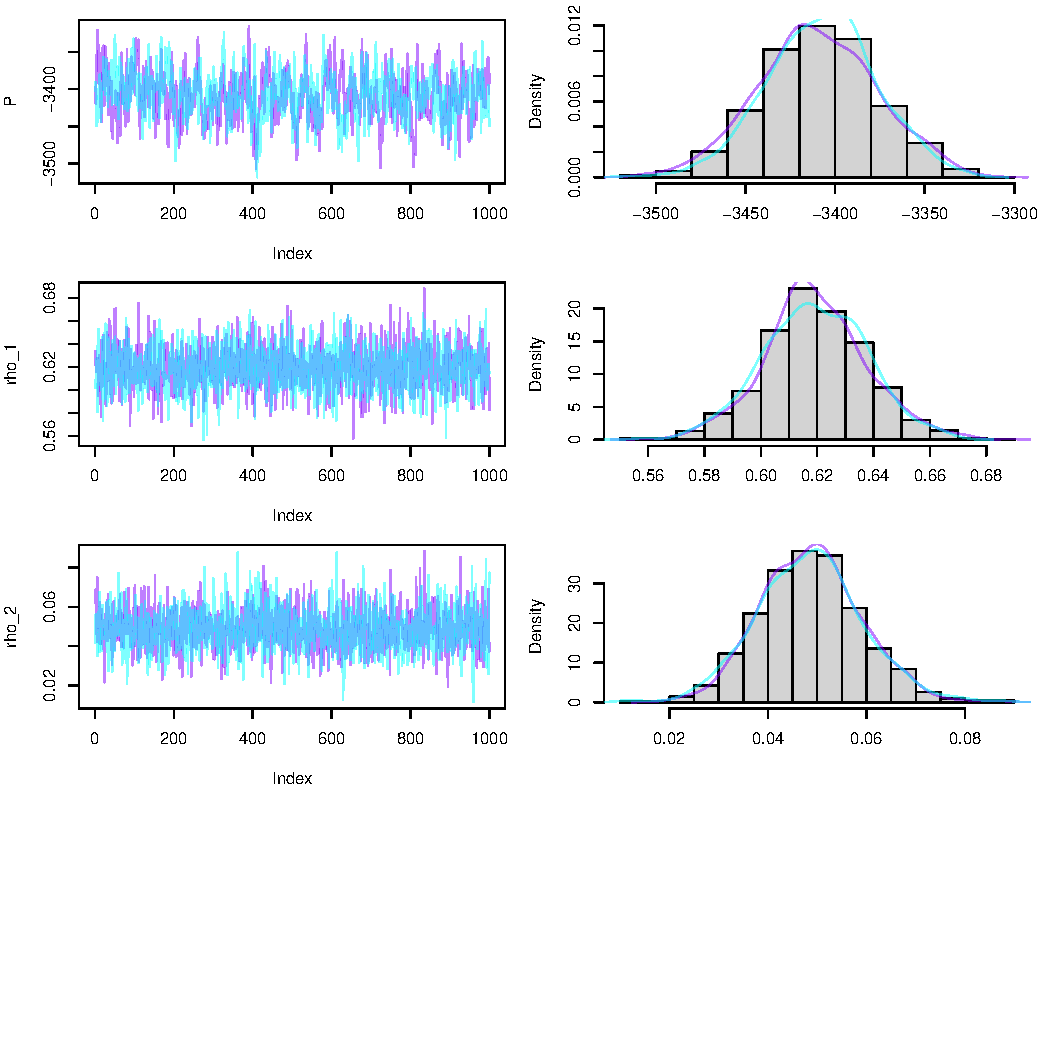
\includegraphics[page=1, width=1\linewidth]{b0_6_2/out_mTL/fig_tracePlot_rho.pdf}
\caption{
    \textbf{Traces of the chains of the correlation parameters of the variance-covariance matrix of the maximum trophic level model.}
    Each row shows samples of a given parameter, sorted by index (left), or shown as a histogram (right).
    $P$ corresponds to the log posterior density of the parameters, $rho_1$ corresponds to the maximum correlation parameter (i.e. $\alpha$ in the main text), and $rho_2$ is the rate of decrease (of the correlation) with distance (i.e. $\beta$ in the main text). 
    These parameters model a decrease in the correlation in the maximum trophic levels, $\rho_{ij}$, of two sites, $i$ and $j$ located in the same hydrographic basin with Euclidean distance, $\rho_{ij} = \alpha \exp\left( - \beta d_{ij}\right)$.
    Samples were obtained by differential-evolution Monte-Carlo sampling of the posterior distribution (\cite{TerBraak2006}).
    Chains were burned by removing the first half of the iterations, and then by taking a thousand evenly spaced samples of the remaining samples.
} 
\end{center}
\end{figure}

%%
\begin{figure}[H]
\begin{center}
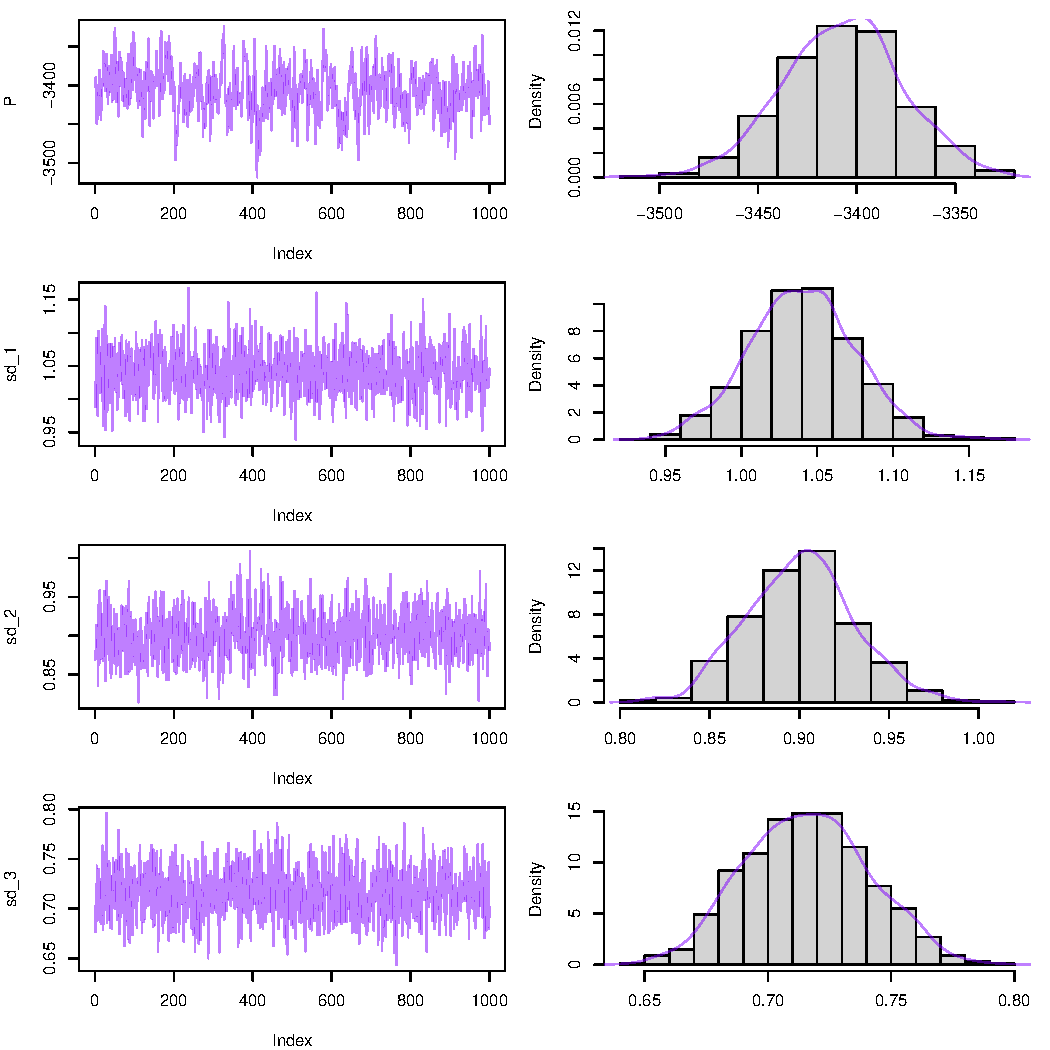
\includegraphics[page=1, width=1\linewidth]{b0_6_2/out_mTL/fig_tracePlot_sd_lik.pdf}
\caption{
    \textbf{Traces of the chains of the variance parameters of the variance-covariance matrix of the maximum trophic level model (1/2).}
    Each row shows samples of a given parameter, sorted by index (left), or shown as a histogram (right).
    $P$ corresponds to the log posterior density of the parameters, $sd_1$ to $sd_7$ correspond to the estimated basin-specific standard deviations of the response variable (i.e. maximum trophic level).
    Our dataset contained seven hydrographic basins, so there are seven estimated basin-specific standard deviations.
    Samples were obtained by differential-evolution Monte-Carlo sampling of the posterior distribution (\cite{TerBraak2006}).
    Chains were burned by removing the first half of the iterations, and then by taking a thousand evenly spaced samples of the remaining samples.
} 
\end{center}
\end{figure}

%%
\begin{figure}[H]
\begin{center}
\includegraphics[page=2, width=1\linewidth]{b0_6_2/out_mTL/fig_tracePlot_sd_lik.pdf}
\caption{
    \textbf{Traces of the chains of the variance parameters of the variance-covariance matrix of the maximum trophic level model (2/2).}
    Each row shows samples of a given parameter, sorted by index (left), or shown as a histogram (right).
    $P$ corresponds to the log posterior density of the parameters, $sd_1$ to $sd_7$ correspond to the estimated basin-specific standard deviations of the response variable (i.e. maximum trophic level).
    Our dataset contained seven hydrographic basins, so there are seven estimated basin-specific standard deviations.
    Samples were obtained by differential-evolution Monte-Carlo sampling of the posterior distribution (\cite{TerBraak2006}).
    Chains were burned by removing the first half of the iterations, and then by taking a thousand evenly spaced samples of the remaining samples.
} 
\end{center}
\end{figure}

%%
\begin{figure}[H]
\begin{center}
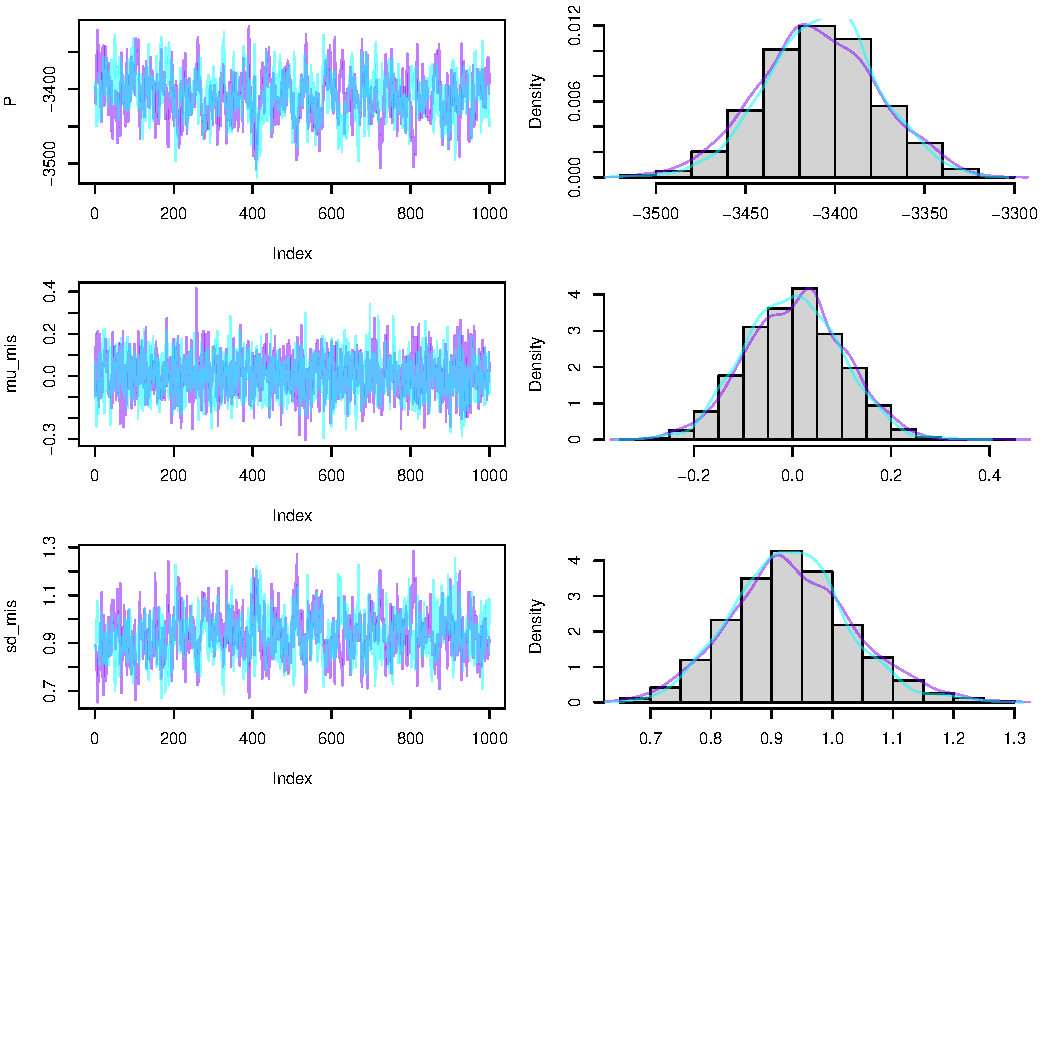
\includegraphics[page=1, width=1\linewidth]{b0_6_2/out_mTL/fig_tracePlot_sd_mis.pdf}
\caption{
    \textbf{Traces of the chains of the parameters of the distribution of missing BOD measurements of the maximum trophic level model.}
    Each row shows samples of a given parameter, sorted by index (left), or shown as a histogram (right).
    $P$ corresponds to the log posterior density of the parameters.
    $mu_{mis}$ and $sd_{mis}$ correspond to the mean and standard deviation of the distribution of the missing BOD observations.
    The distribution of missing BOD measurements is assumed to be a normal distribution.
    Samples were obtained by differential-evolution Monte-Carlo sampling of the posterior distribution (\cite{TerBraak2006}).
    Chains were burned by removing the first half of the iterations, and then by taking a thousand evenly spaced samples of the remaining samples.
} 
\end{center}
\end{figure}

%
%%%

\printbibliography
\end{document} 
